\documentclass[11pt,a4paper]{article}

\usepackage[margin=1in]{geometry}
\usepackage{titlesec}
\usepackage{enumitem}
\usepackage{hyperref}
\usepackage{parskip}
\usepackage{graphicx}
\usepackage{float}
\usepackage{booktabs}
\usepackage{amsmath}

\hypersetup{colorlinks=true, linkcolor=blue, urlcolor=blue}

\titleformat{\section}{\large\bfseries}{\thesection}{0.5em}{}
\titleformat{\subsection}{\normalsize\bfseries}{\thesubsection}{0.5em}{}
\setlist{leftmargin=1.4em, topsep=2pt, itemsep=2pt}

\title{\vspace{-1.5cm}\textbf{PKCERT AI \& Software Development Internship \\ Task 13: Advanced Model Evaluation \& Handling Imbalanced Data}}
\author{Abdullah Amir}
\date{AI and Software Development \\ 20 July 2026}

\begin{document}

\maketitle
\vspace{-0.8cm}

This report covers the theory and the results. The full code, outputs and plots live in
the notebook \texttt{model\_evaluation.ipynb}. The dataset is the \textbf{ULB Credit Card
Fraud Detection} dataset: 284,807 transactions made by European cardholders over two
days in September 2013, of which \textbf{492 are fraudulent}, an imbalance ratio of about
\textbf{578 legitimate transactions for every one fraud}. It is the textbook case for
this task: accuracy is close to worthless on it, and the entire point of ROC-AUC,
learning curves, SMOTE and class weighting is to evaluate and correct for exactly this
kind of imbalance.

% ----------------------------------------------------------------
\section*{Part A: Dataset Selection \& Preparation}

\textbf{What the features are.} Each row is one transaction. \texttt{V1}--\texttt{V28}
are principal components of the original transaction features, released already
PCA-transformed because the underlying features are confidential. Only \texttt{Time}
(seconds since the first transaction in the dataset) and \texttt{Amount} are on their
original scale. \texttt{Class} is the target: 1 for fraud, 0 otherwise.

\textbf{Missing values and scaling.} There are no missing values. \texttt{V1}--\texttt{V28}
arrive already standardised as a side effect of the PCA that produced them, so only
\texttt{Time} and \texttt{Amount} need scaling before a gradient-based model like
Logistic Regression sees them; I fit a \texttt{StandardScaler} on those two columns
using the training fold only, then applied it to the test fold.

\textbf{Split.} An 80/20 train/test split, \textbf{stratified} on \texttt{Class} so both
folds keep the same 0.173\% fraud rate: 394 fraud cases in the 227,845-row training set,
98 in the 56,962-row test set. Stratification matters more than usual here; an unlucky
unstratified split could easily send most of the 492 known frauds to one side.

\begin{figure}[H]
    \centering
    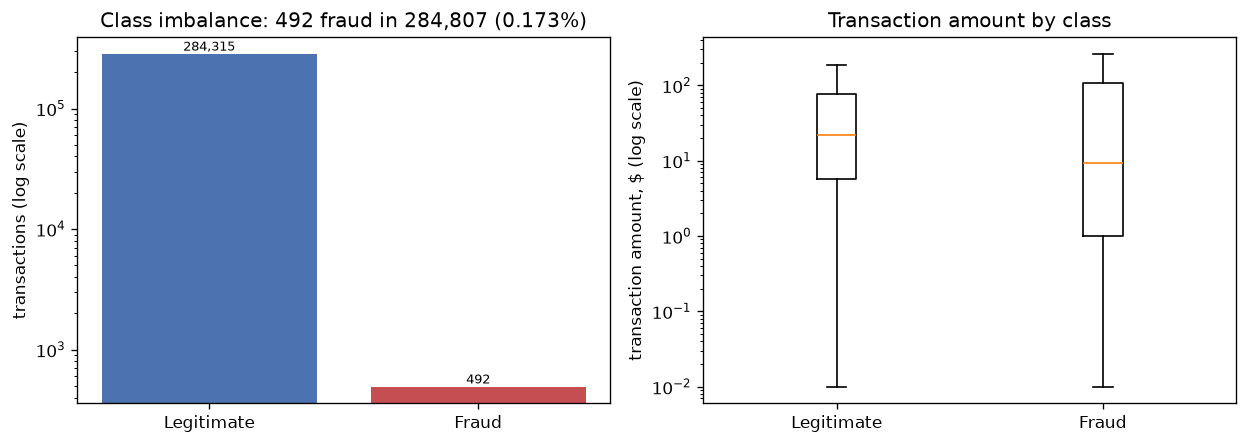
\includegraphics[width=0.95\textwidth]{figures/01_class_imbalance.png}
    \caption{Left: the imbalance itself, log-scaled because a linear axis would render
    the fraud bar invisible. Right: transaction amount by class; fraud amounts have a
    lower median (\$9.25 vs \$22.00) but a heavier tail, which is a real difference
    worth checking rather than assuming fraud simply means ``large transaction.''}
\end{figure}

% ----------------------------------------------------------------
\section*{Part B: Advanced Model Evaluation}

\textbf{The baseline model} is a Logistic Regression trained on the training fold exactly
as it is, with no resampling and no class weighting. Every later comparison in Part C is
measured against it.

\begin{table}[H]
\centering
\begin{tabular}{lrrrrrr}
\toprule
\textbf{Baseline} & \textbf{Acc} & \textbf{Prec} & \textbf{Rec} & \textbf{F1} & \textbf{ROC-AUC} & \textbf{PR-AUC} \\
\midrule
No handling & 0.9992 & 0.8289 & 0.6429 & 0.7241 & 0.9559 & 0.7432 \\
\bottomrule
\end{tabular}
\caption{Baseline Logistic Regression, evaluated on the untouched, imbalanced test set.}
\end{table}

\textbf{Accuracy is meaningless here, and it is worth showing why rather than asserting
it.} A classifier that always predicts ``legitimate'' scores \textbf{99.83\% accuracy}
while catching \textbf{0 of the 98} fraud cases in the test set. The baseline's own
99.92\% accuracy sounds barely better, yet it catches 63 of 98 frauds; accuracy simply
cannot distinguish these two very different classifiers when one class is this rare.

\subsection*{B1. ROC Curve and ROC-AUC}

The \textbf{ROC curve} plots true positive rate against false positive rate as the
decision threshold sweeps from 1 to 0; \textbf{ROC-AUC} is the probability that a
randomly chosen fraud is ranked above a randomly chosen legitimate transaction by the
model's score.

\begin{figure}[H]
    \centering
    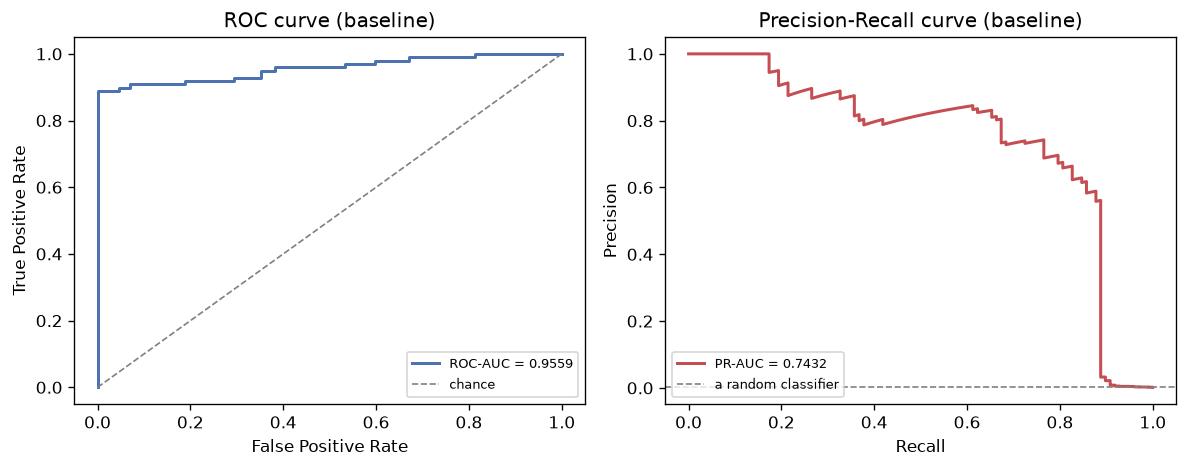
\includegraphics[width=0.95\textwidth]{figures/02_roc_pr_baseline.png}
    \caption{Left: the ROC curve, ROC-AUC 0.9559, which looks close to perfect. Right:
    the Precision-Recall curve for the same model, PR-AUC 0.7432, a far less flattering
    and, for this dataset, more honest picture.}
\end{figure}

\textbf{The ROC-AUC of 0.956 is real but is also flattering in a specific, checkable way.}
The false-positive-rate axis is computed against 56,864 legitimate test transactions, so
even a fairly large number of false positives barely moves it; a model can look excellent
on ROC-AUC while its precision on the rare positive class is falling apart. The
\textbf{Precision-Recall curve}, which never involves the negative class in its
denominator, is the sharper instrument for a dataset this imbalanced, and its PR-AUC of
0.743 is the number I trust more when the two disagree.

\subsection*{B2. Learning Curve}

The learning curve tracks ROC-AUC on the training fold and on 5-fold cross-validation as
the training set grows, which is how you tell underfitting, overfitting and
generalisation apart instead of guessing from one final score.

\begin{figure}[H]
    \centering
    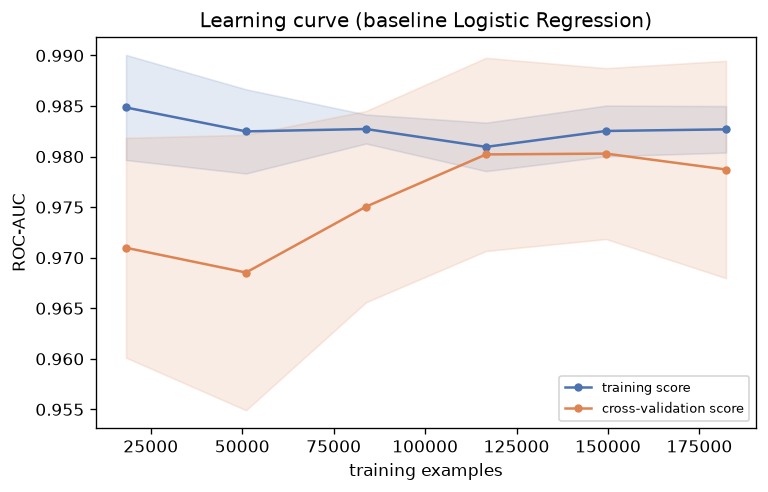
\includegraphics[width=0.72\textwidth]{figures/03_learning_curve.png}
    \caption{Training and cross-validation ROC-AUC converge to within about 0.004 of each
    other by the full training set, with the gap shrinking rather than growing as more
    data is added.}
\end{figure}

\textbf{Reading it plainly:} both curves sit high throughout (0.97--0.99), which rules
out underfitting -- the model is not too weak for the problem. The gap between them
starts at 0.014 with the smallest slice of data and narrows to 0.004 at the full training
set, which rules out overfitting too -- a genuinely overfit model would show that gap
\emph{widening} as it is given more room to memorise. What this curve actually shows is a
well-fit model that \textbf{generalises}, with cross-validation score still edging upward
through most of the range, meaning more labelled fraud examples would likely help a
little further, though the curve is close to flat by the end.

% ----------------------------------------------------------------
\section*{Part C: Handling Imbalanced Data}

\subsection*{C1. The imbalance}

In the training fold alone: \textbf{227,451 legitimate transactions against 394 fraud},
0.173\% positive, identical to the full dataset's ratio thanks to stratification. Two
techniques were applied to this training fold, and both were evaluated on the same
untouched, imbalanced test fold used for the baseline, so the three rows below are
directly comparable.

\subsection*{C2. SMOTE}

\textbf{SMOTE} (Synthetic Minority Oversampling Technique) generates new fraud examples
by interpolating between each real fraud case and its nearest fraudulent neighbours,
applied to the training data only, until the classes are balanced at 227,451 each.

\begin{figure}[H]
    \centering
    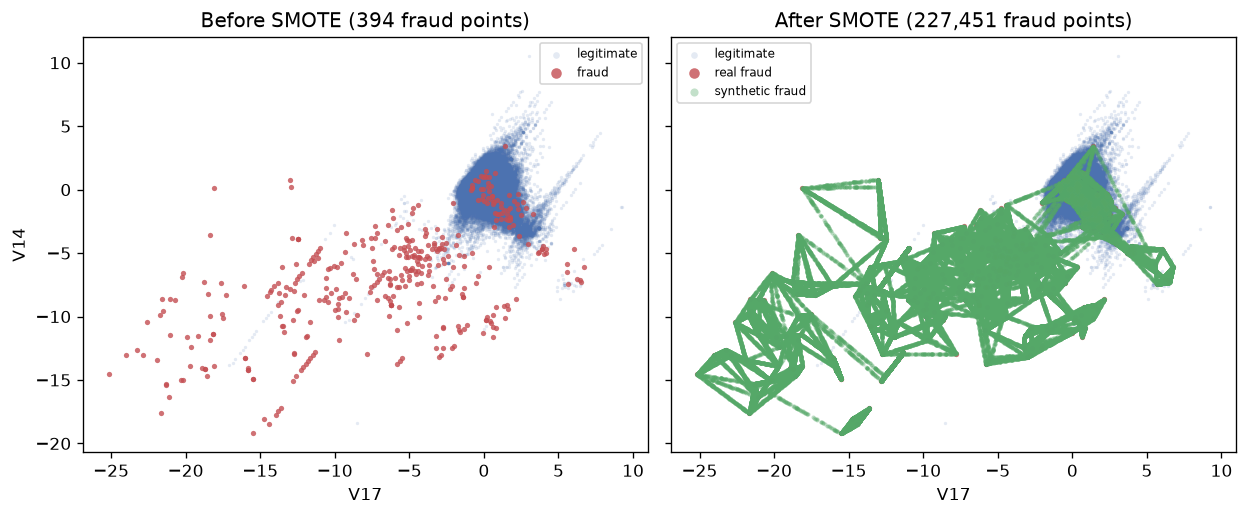
\includegraphics[width=0.95\textwidth]{figures/04_smote_effect.png}
    \caption{The two features most correlated with fraud, V17 and V14. Left: the 394 real
    fraud points before SMOTE. Right: after SMOTE, with the synthetic points visibly
    tracing straight lines between real frauds and their neighbours, the triangulated web
    that interpolation produces.}
\end{figure}

The picture is a useful caution on its own: \textbf{SMOTE cannot invent structure that
was not already present in the 394 real training frauds}; it can only interpolate between
them, which is why the synthetic cloud never leaves the convex hull the real points
already occupied.

\subsection*{C3. Class weighting}

\textbf{Class weighting} reweights the loss function directly
(\texttt{class\_weight='balanced'}), making a missed fraud cost roughly 578 times more
than a missed legitimate transaction during training, without generating any new rows or
touching the test set.

\begin{table}[H]
\centering
\begin{tabular}{lrrrrrr}
\toprule
\textbf{Method} & \textbf{Acc} & \textbf{Prec} & \textbf{Rec} & \textbf{F1} & \textbf{ROC-AUC} & \textbf{PR-AUC} \\
\midrule
Original (no handling) & 0.9992 & 0.8289 & 0.6429 & 0.7241 & 0.9559 & 0.7432 \\
SMOTE & 0.9742 & 0.0580 & \textbf{0.9184} & 0.1092 & 0.9699 & 0.7249 \\
Class weighting & 0.9755 & 0.0610 & \textbf{0.9184} & 0.1144 & \textbf{0.9722} & 0.7159 \\
\bottomrule
\end{tabular}
\caption{All three evaluated on the same untouched, imbalanced test set (56,864
legitimate, 98 fraud).}
\end{table}

\begin{figure}[H]
    \centering
    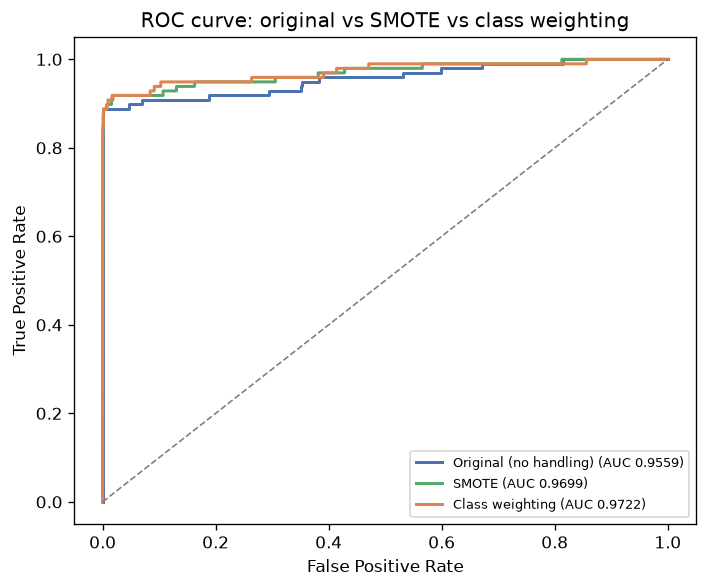
\includegraphics[width=0.68\textwidth]{figures/05_roc_comparison.png}
    \caption{ROC curves for all three. SMOTE and class weighting both sit slightly above
    the baseline, but the ROC curve alone hides the story the table above tells.}
\end{figure}

\begin{figure}[H]
    \centering
    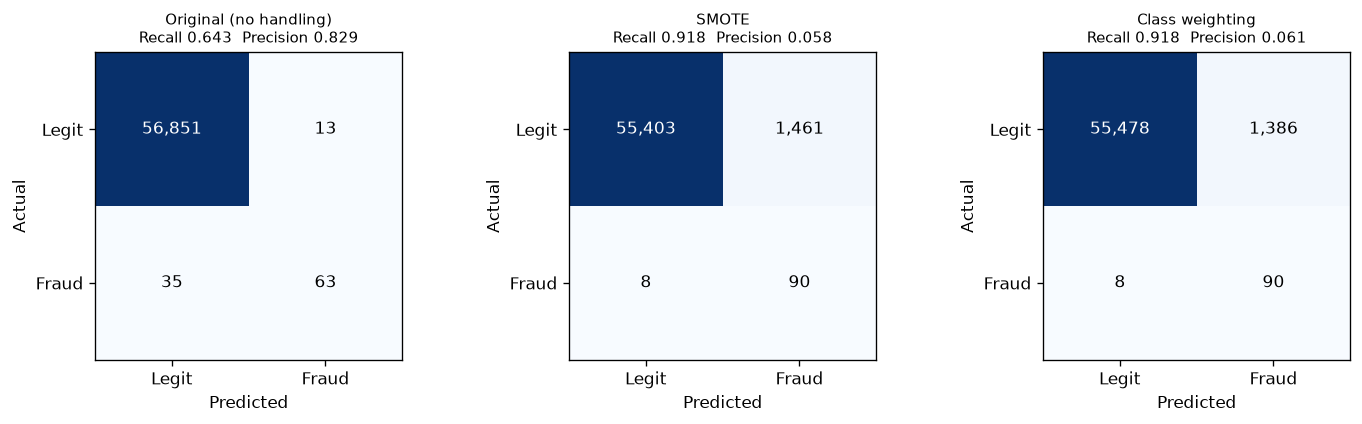
\includegraphics[width=0.95\textwidth]{figures/06_confusion_matrices.png}
    \caption{Confusion matrices side by side. Both SMOTE and class weighting catch 90 of
    98 frauds against the baseline's 63, but SMOTE does it by flagging 1,461 legitimate
    transactions as fraud and class weighting by flagging 1,386 -- against the baseline's
    13.}
\end{figure}

\textbf{Three results here, and none of them is the naive story.}

\textbf{First, both techniques roughly triple recall (0.643 to 0.918) but F1 gets
substantially worse, not better} (0.724 to about 0.11). It would have been easy to
report only ROC-AUC, watch it tick up from 0.956 to 0.97, and call both techniques a
straightforward win. Looking at precision and F1 instead shows the real trade: the
extra 27 frauds caught cost over a hundred times more false alarms, from 13 to well over
a thousand.

\textbf{Second, PR-AUC -- the one metric here that does not depend on the 0.5 decision
threshold -- is actually highest for the untouched baseline} (0.743) and slightly
\emph{lower} for both SMOTE (0.725) and class weighting (0.716). Neither technique
improved the model's underlying ability to rank a fraud above a legitimate transaction;
what they did was move where the default threshold sits on a ranking that was already
about as good as it was going to get. That is a genuinely different claim from ``SMOTE
improves the model,'' and only shows up if PR-AUC is checked alongside ROC-AUC rather
than instead of it.

\textbf{Third, class weighting beats SMOTE outright on this comparison}: identical recall
(90/98 caught either way) with fewer false positives (1,386 against 1,461), no synthetic
data, and no extra computation for generating it. There was no reason to expect this in
advance -- SMOTE is the more elaborate technique -- but the simpler one wins here.

% ----------------------------------------------------------------
\section*{Part D: Comparative Analysis \& Recommendation}

\begin{table}[H]
\centering
\begin{tabular}{lp{5.6cm}p{5.6cm}}
\toprule
\textbf{Method} & \textbf{Strength} & \textbf{Weakness} \\
\midrule
Original & Best precision (0.829) and F1 (0.724); cheapest to train & Misses 35 of 98 frauds \\
SMOTE & Best recall alongside class weighting (0.918) & Worst precision (0.058); synthetic data can only interpolate known frauds \\
Class weighting & Same recall as SMOTE with better precision; free, no synthetic rows & Still floods the review queue with false positives \\
\bottomrule
\end{tabular}
\caption{The trade-off in one table.}
\end{table}

\textbf{Recommendation.} For this dataset, \emph{class weighting is the better of the two
imbalance-handling techniques}: it matches SMOTE's recall with fewer false positives and
no synthetic data to trust. But neither should mechanically replace the untouched
baseline -- the correct choice is a business decision about which error is more
expensive. If a missed fraud costs far more than a manually reviewed false alarm, the
usual case in fraud detection, class weighting's recall of 0.918 is worth its precision
of 0.061. If false positives carry a real cost of their own, such as blocking genuine
customers at checkout, the baseline's precision of 0.829 may be the safer choice, or the
two could be blended by moving the baseline's own decision threshold rather than
resampling at all, since Part B2 already showed its underlying ranking (PR-AUC 0.743) is
the best of the three on offer.

\textbf{The caveat that matters most.} The test set contains only \textbf{98 fraud cases},
so every precision and recall figure in this report moves in steps of roughly one
percentage point per transaction, and a different random split could plausibly shift the
recall count by one or two frauds in either direction. The direction of every finding
above is solid -- SMOTE and class weighting trade precision for recall, class weighting
edges out SMOTE, PR-AUC does not improve -- but the third decimal place in any of these
numbers should not be over-trusted.

\textbf{Conclusion.} The thread running through this task is that no single metric tells
the whole story on an imbalanced dataset. Accuracy said the baseline was excellent and
was nearly uninformative. ROC-AUC said SMOTE and class weighting were improvements and
was, at best, incomplete: PR-AUC says the model's ranking did not actually get better,
only the threshold's position on it. F1 said the resampled models were worse, which
accuracy and ROC-AUC alone would never have shown. The learning curve was the one
piece of good news that needed no caveat: the model is neither underfit nor overfit, and
more labelled fraud would likely help further. Reading several metrics against each
other, rather than picking the one that looks best, was the actual work of this task.

\vspace{0.4cm}
\noindent The notebook and README are on GitHub: {\small\scalebox{0.82}[1]{\url{https://github.com/AbdullahAmir06/ai-internship-abdullahamir}}}

\end{document}